\documentclass{article}
\usepackage[utf8]{inputenc}
\usepackage{
    geometry, 
    tocloft, 
    siunitx, 
    amssymb,
    amsmath,
    graphicx, 
    float, 
    setspace,  
    bm, 
    titlesec, 
    booktabs,
    caption,
    subcaption,
    listings,
    bigints,
    fancyhdr,
    algorithm,
    algpseudocode
}
\usepackage[T1]{fontenc}

% establish page form and margins
\geometry{a4paper}
% add double line spacing
\doublespacing
% paragraph styling
\setlength{\parindent}{0ex}
\setlength{\parskip}{1em}

% headers on each page
\pagestyle{fancy}
\fancyhf{}
\rhead{Jason Wang (1008584649)}
\lhead{CSC258 Assembly Project Report (29 March 2023)}

\begin{document}




\begin{center}
        \huge
        CSC258 Assembly Project Report        \vspace{1cm}
        
        % \large
        % \textbf{Research Question:}
        
        % To what extent are different approaches to the hyperparameter tuning of a Random Forest Classifier effective in improving accuracy in predicting credit card fraud?
        \large
        Jason Wang (1008584649)
        
        29 March 2023

       

 \end{center}
 
 \tableofcontents
 
 
 
\vspace{10mm}

\addcontentsline{toc}{section}{Milestone 1}
\section*{Milestone 1}


\addcontentsline{toc}{subsection}{Constants and Variables}
\subsection*{Constants and Variables}

The following are the constants defined in memory:
\begin{enumerate}
	\item\texttt{DISPLAY\_WIDTH = 256} (width of display in pixels)
	\item\texttt{DISPLAY\_HEIGHT = 256} (height of display in pixels)
	\item\texttt{ADDR\_DSPL = 0x10008000} (address of the bitmap display)
	\item\texttt{ADDR\_KBRD = 0xffff0000} (address of the keyboard)
	\item\texttt{BG\_COLOUR = 0x000000} (colour code of the background)
	\item\texttt{FRAME\_TIME = 60} (sleep time between frames in ms)
	\item\texttt{HEART\_ADDR = [520, 556, 592]} (offset from \texttt{ADDR\_DSPL} of the top left corner for each heart)
	\item\texttt{HEART\_FULL\_COLOUR = 0xe54b4b} (colour of heart when full)
	\item\texttt{HEART\_EMPTY\_COLOUR = 0x000000} (colour of heart when life is lost)
	\item\texttt{SCORE\_ADDR = [716, 732, 748]} (offset from \texttt{ADDR\_DSPL} of the top left corner for each digit of the score)
	\item\texttt{WALL\_COLOUR = 0x555555} (colour of the walls)
	\item\texttt{TOP\_WALL\_THICKNESS = 36} (thickness of the top wall)
	\item\texttt{SIDE\_WALL\_THICKNESS = 8} (thickness of the side walls)
	\item\texttt{BRICK\_COLOUR = 0x82d2c8} (colour for the breakable bricks)
	\item\texttt{BRICK\_ROWS = 28} (thickness of the row of bricks)
	\item\texttt{BRICK\_START\_HEIGHT = 56} (starting height of the brick row)
	\item\texttt{BRICK\_WIDTH = 16} (width of an individual brick)
	\item\texttt{BRICK\_HEIGHT = 8} (height of an individual brick)
	\item\texttt{PADDLE\_COLOUR = 0xeeeeee} (colour code of the paddle)
	\item\texttt{PADDLE\_WIDTH = 36} (width of the paddle)
	\item\texttt{PADDLE\_HEIGHT = 4} (height o the paddle)
	\item\texttt{BALL\_COLOUR = 0xe54b4b} (colour code of the ball)
	\item\texttt{BALL\_SIZE = 4} (width and height of the ball)
\end{enumerate}
The following are the variables defined in memory as well as their initial values:
\begin{enumerate}
	\item\texttt{PADDLE\_X = 112} (x coordinate of the top left corner of the paddle)
	\item\texttt{PADDLE\_Y = 252} (y coordinate of the top left coordinate of the paddle)
	\item\texttt{BALL\_X = 128} (x coordinate of the ball)
	\item\texttt{BALL\_Y = 228} (y coordinate of the ball)
	\item\texttt{BALL\_VX = -4} (x velocity of the ball)
	\item\texttt{BALL\_VY = -4} (y velocity of the ball)
	\item\texttt{IS\_PAUSED = 0} (boolean indicating whether the game is paused or not)
	\item\texttt{IS\_LAUNCHING = 1} (boolean indicating whether the user is currently positioning the ball)
	\item\texttt{LIVES = 3} (number of lives)
\item\texttt{SCORE = 0} (current score measured by bricks broken)
\end{enumerate}


\pagebreak

\addcontentsline{toc}{subsection}{Scene}
\subsection*{Scene}

\begin{figure}[H]
    \centering
    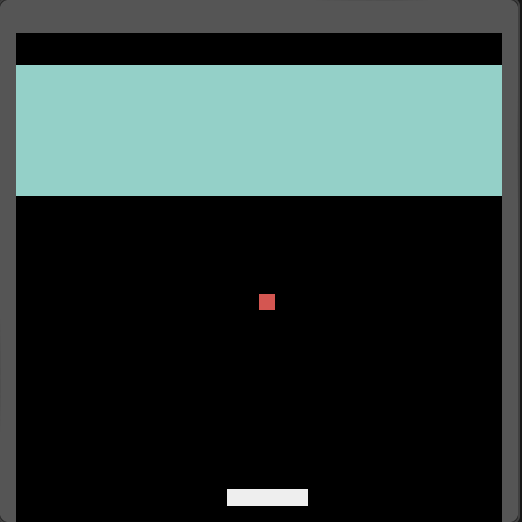
\includegraphics[width=1\textwidth]{media/milestone1_static}
    \caption{Screenshot of the static scene developed in Milestone 1}
    \label{fig:fig1}
\end{figure}


\pagebreak


\addcontentsline{toc}{section}{Milestone 3}
\section*{Milestone 3}

\textbf{How will the ball change directions when it collides?}

Depending on the direction in which the collision occurs, the ball's parallel velocity component will be inverted. That is, if the pixel $(\texttt{BALL\_X}+\texttt{BALL\_VX}, \,\texttt{BALL\_Y})$ has a colour determined to be collidable, the ball reacts to a collision in the x-direction by reversing the x-velocity
\[\texttt{BALL\_VX} = -\texttt{BALL\_VX}\]
and if $(\texttt{BALL\_X},\,\texttt{BALL\_Y}+\texttt{BALL\_VY})$ has a colour determined to be a collidable object, the ball reacts to this collision in the y-direction by reversing the y-velocity
\[\texttt{BALL\_VY} = -\texttt{BALL\_VY}\]
If the ball collides with a corner (whether it be the inward or outward corner), which occurs when both of the above cases are true, the ball will reverse direction completely:
\[\texttt{BALL\_VX} = -\texttt{BALL\_VX}; \,\texttt{BALL\_VX} = -\texttt{BALL\_VX}\]


\pagebreak
\addcontentsline{toc}{section}{How to Play}
\section*{How to Play}

Ensure that the bitmap display is configured to 256x256 with 4px unit size.

\textbf{Controls:}
\begin{itemize}
	\item <a> + <d>: move paddle left and right
	\item <space>: launch ball when starting an attempt
	\item <p>: pause the game
	\item <q>: quit the game
\end{itemize}
Launch the ball with <space> and then destroy all the bricks to win! If the ball reaches the bottom of the screen, a life will be lost. After three lives lost, the game will end.


















\end{document}